%Af: Søren (?)
%1st review: Troels
%2nd review Morten
\subsection{Toolchain}
When programming for the Arduino, it is possible to use the Arduino IDE, developed by the Arduino company.
This IDE uses a specific version of the GCC compiler, which targets the AVR microcontrollers.
The C or C++ code is first checked for errors and compiled to object code, which then is linked with the standard Arduino libraries and any custom libraries.
The linked object code is then compiled to a single Intel Hex file, which is loaded onto the Arduino using the bootloader already situated on the microcontroller.
A USB to serial converter is also implemented directly on most of the Arduino boards, since it is through the serial connection that the microcontroller communicates. 
This toolchain is also shown on \myref{fig:arduino_flow}.\cite{2015ArduinoToolchain}

\tikzfigure{ArduinoFlowDiagram}{Flow diagram showing the flow of the source files onto the Arduino}{arduino_flow}

\noindent
To show how to upload code to an Arduino, some screenshots have been taken to show how this is done through the Arduino IDE.
First to upload any code to the Arduino, the kind of Arduino being used has to be specified, and how to do this can be seen on \myref{fig:choose_arduino}.

Secondly the Port where the Arudino being uploaded to is plugged in needs to be specified, and a screenshot of this can be seen on figure \myref{fig:choose_port}.

When the code is ready to be uploaded to the Arduino a simple press of the arrow in the top of the IDE will upload and run the code. 
This can be seen on figure \myref{fig:serial_monitor}, the code being run on this screenshot is a simple program which turns on an LED on pin 13 of the Arduino with a varying delay, which is also printed to the serial monitor.
The serial monitor is of great use when debugging with the Arduino as it makes it possible to know what values different variables of the program have at run-time.

The code is split into three parts.
The function \texttt{setup()} is run once when the program starts, and here is where different pins are often set to be input or output.
The function \texttt{loop()} is then run continuously as long as the Arduino is turned on. 
The last part in this example is a global variable \texttt{int i} which is set to global in this very simple example.

It is of course also possible to program in many other languages for the Arduino as long as a compiler which compiles for the AVR processors is used.
An example of this could be Java.
NanoVM is an implementation of some of the Java virtual machine for the AVR processors, it does not contain all of its features because of the limited resources the microcontrollers possesses. 
According to the creator NanoVM, see \cite{NanoVM}, will never contain all the features of the JVM, and C is still a much more powerful language when working with microcontrollers. 

Therefore Arduinos own IDE is the one used for the development of the protocol.

\begin{figure}[!ht]
    \begin{subfigure}{0.47\linewidth}
        \centering
        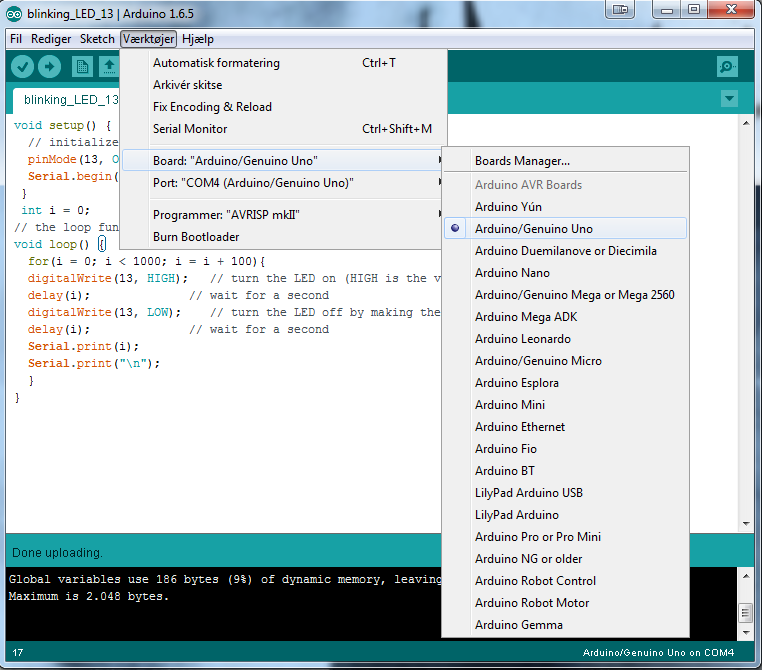
\includegraphics[width=\linewidth]{Figures/ChooseArduino.png}
        \caption{Choose Arduino}
        \label{fig:choose_arduino}
    \end{subfigure}\hfill
    \begin{subfigure}{0.47\linewidth}
        \centering
        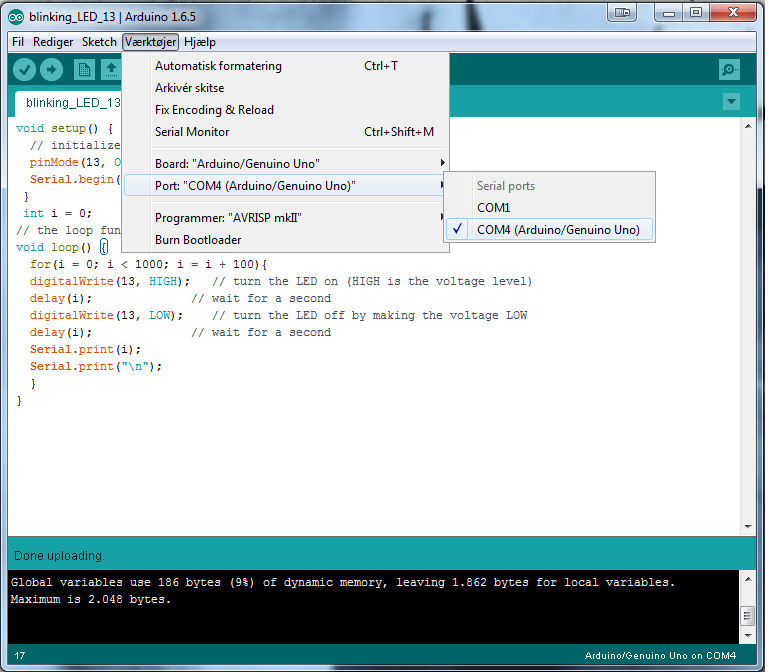
\includegraphics[width=\linewidth]{Figures/ChoosePort.png}
        \caption{Choose Port}
        \label{fig:choose_port}
    \end{subfigure}\\[1ex]
    \begin{subfigure}{\linewidth}
        \centering
        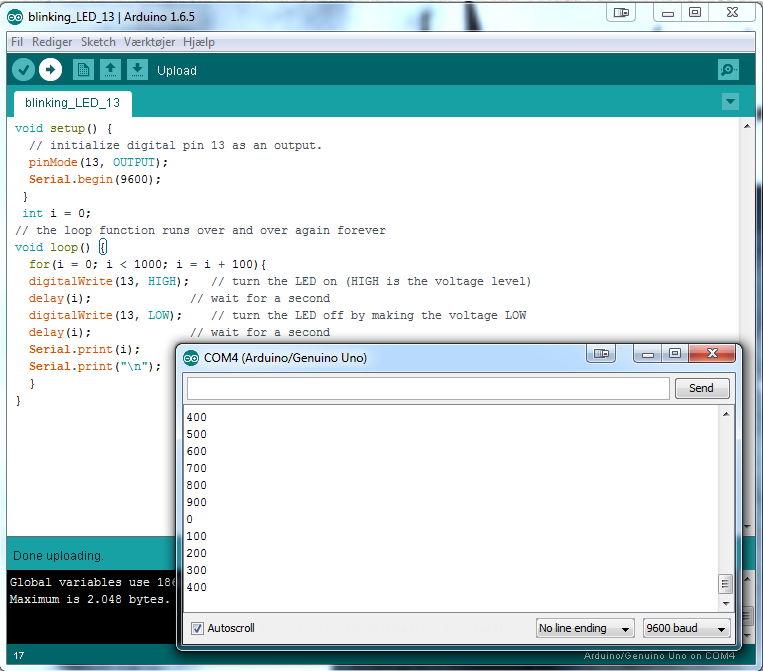
\includegraphics[width=0.47\linewidth]{Figures/SerialMonitor}
        \caption{Serial monitor after uploading code}
        \label{fig:serial_monitor}
    \end{subfigure}
    \caption{Screenshots from the Arduino IDE.}
    \label{fig:ArduinoScreenshots}
\end{figure}
